\documentclass{standalone}
\usepackage{tikz}
\begin{document}
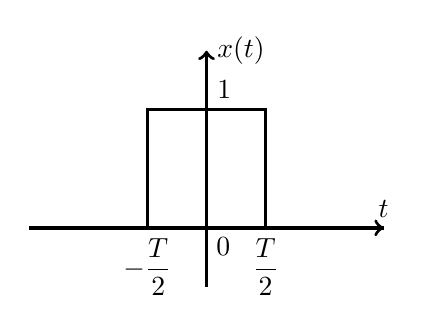
\begin{tikzpicture}[scale=1.5]
    \draw[->,very thick](-1.5,0)--(1.5,0)node[above]{$t$};
    \draw[->,very thick](0,-0.5)--(0,1.5)node[right]{$x(t)$};
    \node[below right]at(0,0){$0$};

    \draw[-,very thick](-1.5,0)--(-0.5,0)node[below]{$\displaystyle-\frac{T}{2}$}--(-0.5,1)--(0,1)node[above right]{$1$}--(0.5,1)--(0.5,0)node[below]{$\displaystyle\frac{T}{2}$}--(1.5,0);        
\end{tikzpicture}
\end{document}